\documentclass[12pt]{article}
\usepackage{csvsimple}
\usepackage[utf8]{inputenc}
\usepackage[left=2cm, top=2cm, text={17cm, 24cm}]{geometry}
\usepackage{times}
\usepackage{verbatim}
\usepackage{multicol}
\usepackage{enumitem}
\usepackage{graphicx} % vkládání obrázků
\usepackage{subfiles}


\begin{document}
    \begin{titlepage}
        \begin{center}
            
\includegraphics[width=0.77\linewidth]{img/fit_logo.png} \\
            \vspace{\stretch{0.4}}        
            \Huge{Projektová dokumentace} \\
            \Large{\textbf{Implementace překladače imperativního jazyka IFJ23}} \\
            \Large{Tým xhrubo01, varianta TRP-izp} \\ 
            \vspace{\stretch{0.6}}
        \end{center}
        \begin{minipage}{0.4 \textwidth}
			{\Large \today}
		\end{minipage}
		\hfill
		\begin{minipage}[r]{0.6 \textwidth}
			\normalsize
            \begin{flushright}
                \begin{tabular}{l l l}
    				Dominik Borek & (xborek12) & 25\%\\
    				\textbf{Ondřej Hruboš} & \textbf{(xhrubo01)} & 25\%\\
    				Radek Jestřabík & (xjestr04)  & 25\%\\
    				Ondřej Šatinský & (xsatin03)  & 25\%\\
    			\end{tabular}
            \end{flushright}
		\end{minipage}
      \newpage
    \end{titlepage}

%Obsah
\begin{center}
\renewcommand{\contentsname}{Obsah}
    \tableofcontents
    \clearpage
\end{center}
 
\section{Úvod}
Cílem projektu do předmětu formalní jazyky a překladače (ifj) bylo vytvoření programu v jazyce C, který načte zdrojový kód zapsaný ve zdrojovém jazyce IFJ23 a přeloží jej do cílového jazyka IFJcode23. Jazyk IFJ23 je zjednodušenou podmnožinou jazyka Swift. 
\\  \\
Bude se jednat o konzolovou aplikaci. Překladač bude načítat řídící program ze standardního vstupu a generovat výsledný kód IFJcode23 na standardní výstup. V případě chyby se chybové hlášení vypíše na standardní výstup.

\section{Návrh a Implementace}
Implementace je provedena pomocí jednotlivých, po sobě jdoucích částí, které jsou detailně popsány v následujících podkapitolách. Mezi tyto části patří: Lexikální analýza, Syntaktická analýza, Sémantická analýza, Generátor vnitřního kódu a Generátor cílového kódu. 

\subsection{Lexikální analýza}
\subfile{sections/scanner.tex}
\subsubsection{Diagram konečného automatu}
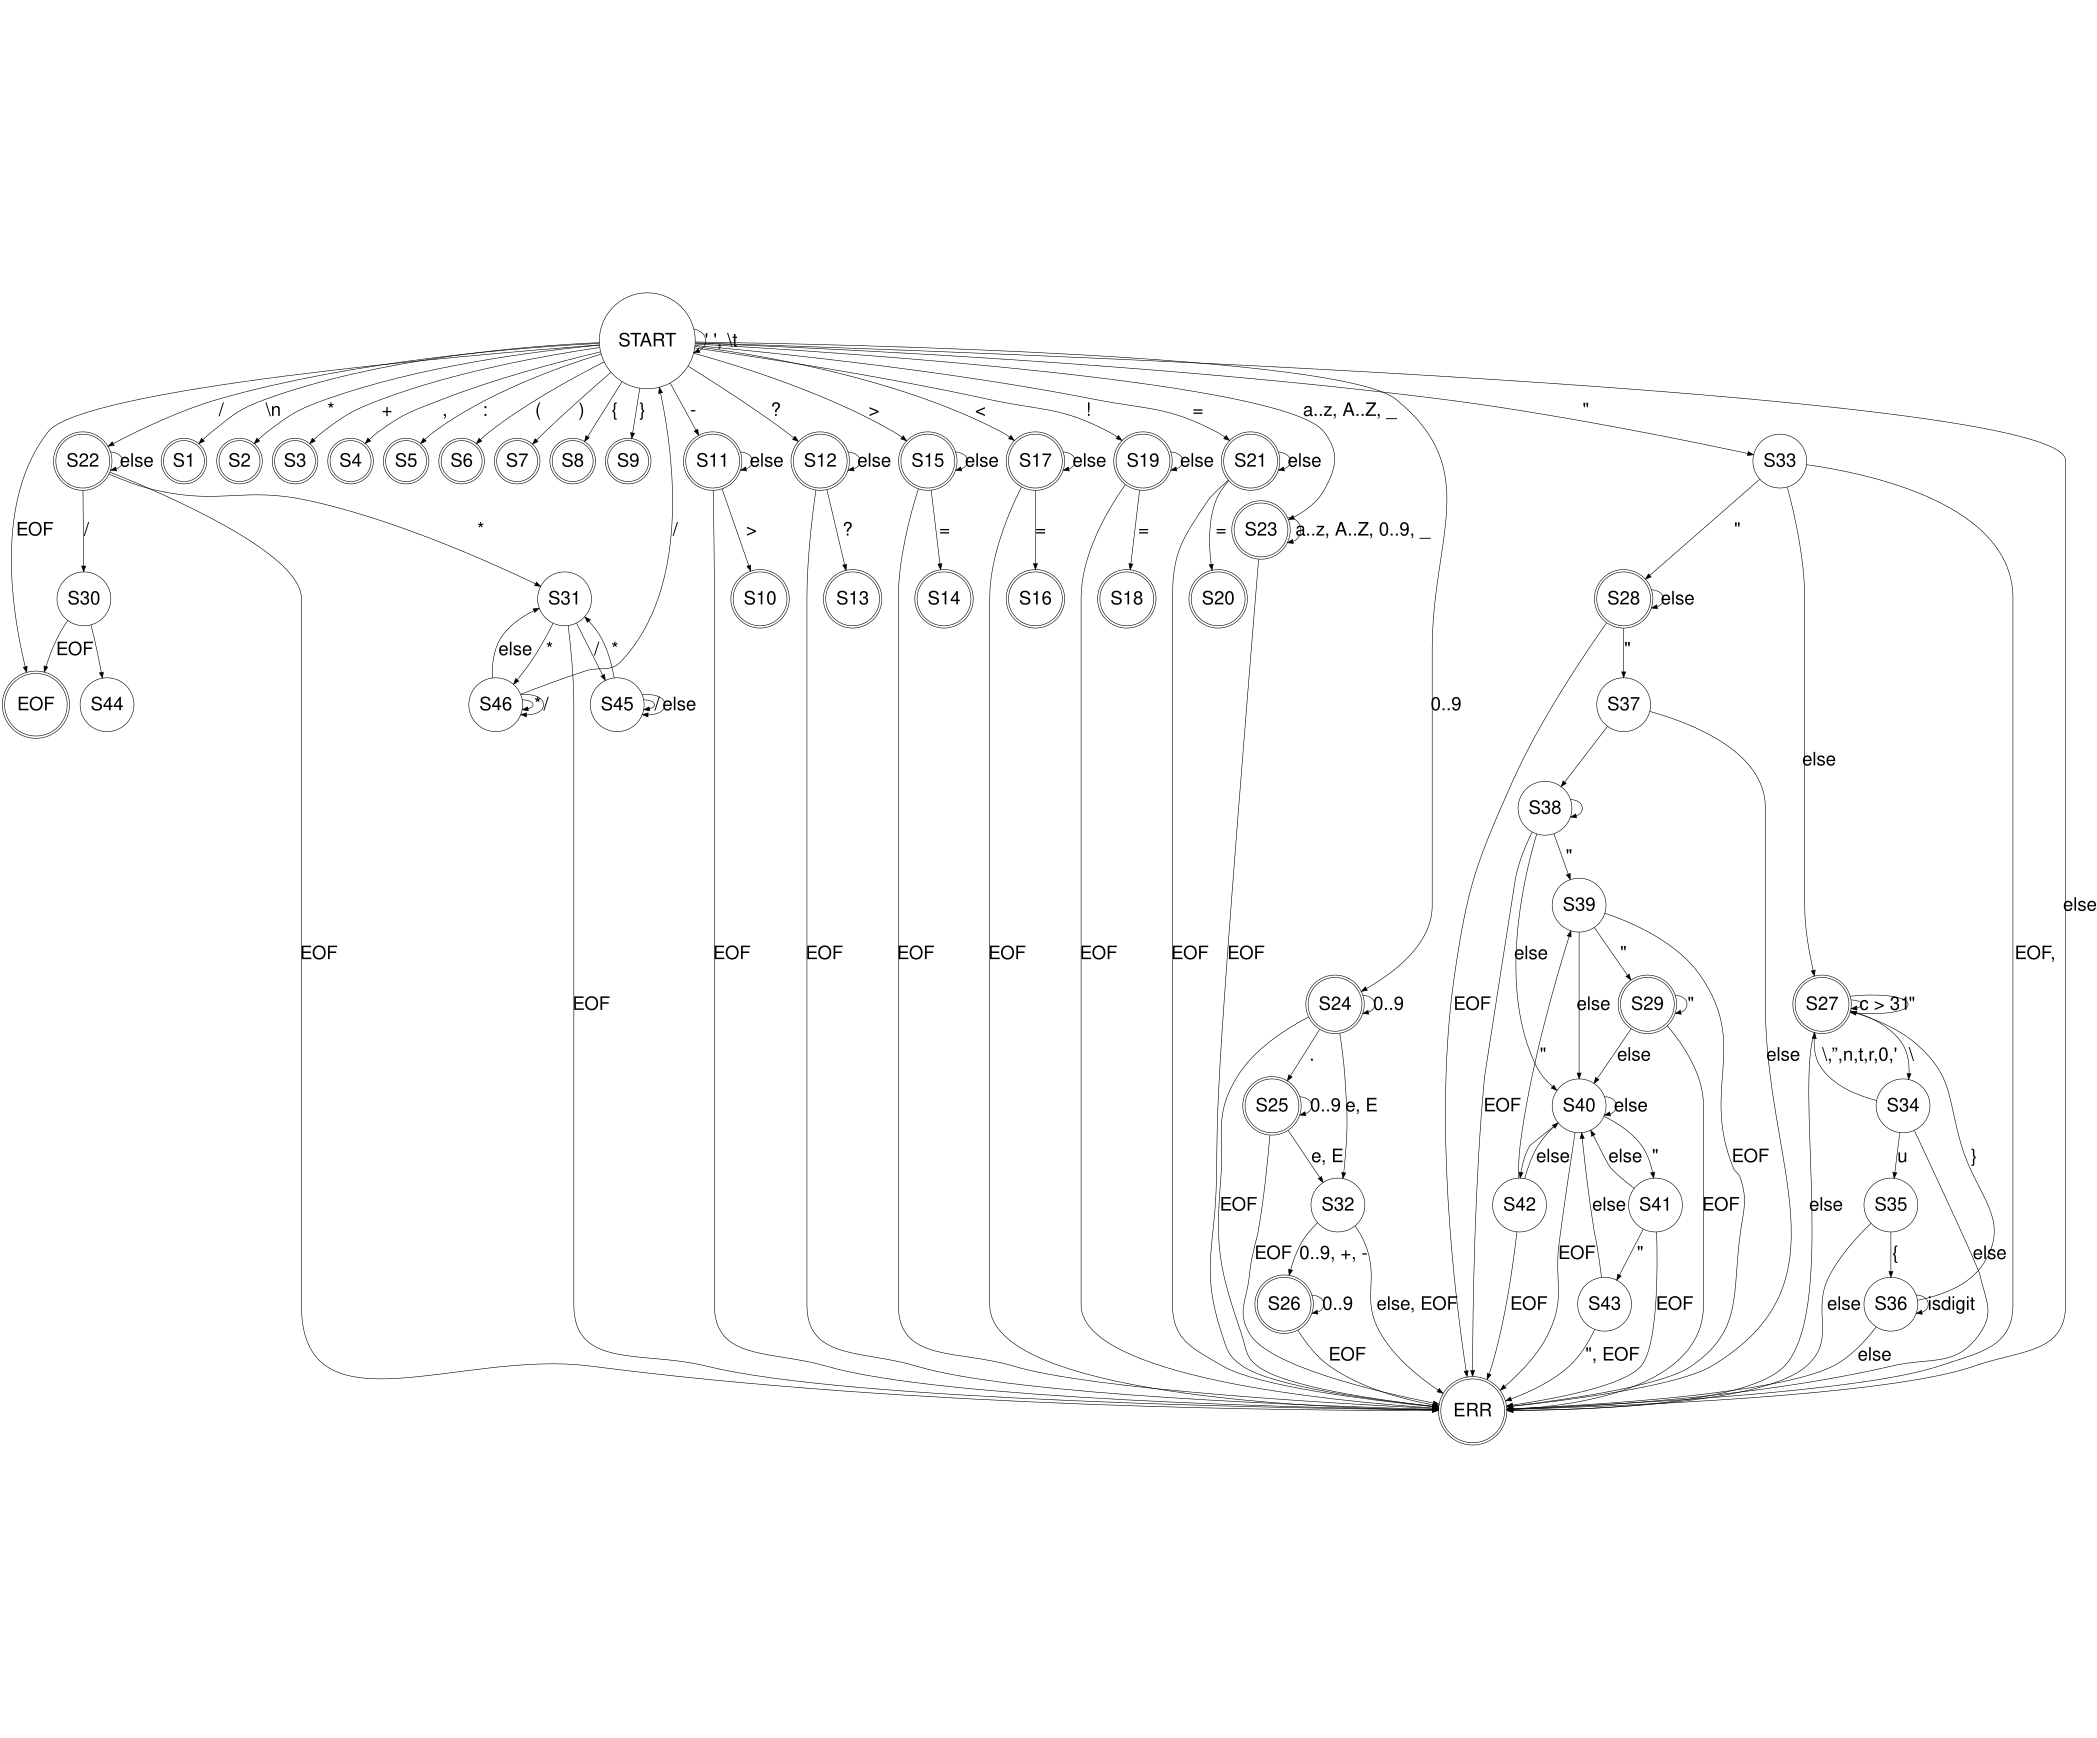
\includegraphics{img/ifj-fsm.png}
\\
\textbf{Legenda stavů:}\\
\begin{tiny}
    \begin{multicols}{2}
    STATE\_START = START\\
    ERR = ERR\\
    NEWLINE = S1\\
    TOKENTYPE\_STAR = S2\\
    TOKENTYPE\_PLUS = S3\\
    TOKENTYPE\_COMMA = S4\\
    TOKENTYPE\_COLON = S5\\
    TOKENTYPE\_PAR\_L = S6\\
    TOKENTYPE\_PAR\_R = S7\\
    TOKENTYPE\_BRACE\_L = S8\\
    TOKENTYPE\_BRACE\_R = S9\\
    TOKENTYPE\_ARROW = S10\\
    STATE\_MINUS = S11\\
    STATE\_QUESTION = S12\\
    TOKENTYPE\_QUESTIONMARK2 = S13\\
    TOKENTYPE\_GREATER\_OR\_EQUAL = S14\\
    STATE\_GREATER = S15\\
    TOKENTYPE\_LESSER\_OR\_EQUAL = S16\\
    STATE\_LESSER = S17\\
    TOKENTYPE\_NOT\_EQUALS = S18\\
    STATE\_EXCLAMATION = S19\\
    TOKENTYPE\_EQUALS2 = S20\\
    STATE\_EQUALS = S21\\
    STATE\_SLASH = S22\\
    STATE\_IDENTIF = S23\\
    STATE\_NUMBER = S24\\
    STATE\_NUMBER\_DOT = S25\\
    STATE\_NUMBER\_EXPONENT = S26\\
    STATE\_STRING\_BODY = S27\\
    STATE\_STRING\_EMPTY = S28\\
    STATE\_STRING\_3\_BODY\_QUOTE2 = S29\\
    STATE\_COMMENT\_LINE = S30\\
    STATE\_COMMENT\_BLOCK = S31\\
    STATE\_NUMBER\_E = S32\\
    STATE\_STRING = S33\\
    STATE\_STRING\_BODY\_SLASH = S34\\
    STATE\_STRING\_BODY\_U = S35\\
    STATE\_STRING\_BODY\_U\_B = S36\\
    STATE\_STRING\_3 = S37\\
    STATE\_STRING\_3\_BODY\_NEWLINE\_0 = S38\\
    STATE\_STRING\_3\_BODY\_QUOTE = S39\\
    STATE\_STRING\_3\_BODY = S40\\
    STATE\_STRING\_3\_BODY\_INV\_QUOTE = S41\\
    STATE\_STRING\_3\_BODY\_NEWLINE = S42\\
    STATE\_STRING\_3\_BODY\_INV\_QUOTE2 = S43\\
    TOKENTYPE\_NEWLINE = S44\\
    STATE\_COMMENT\_BLOCK\_SLASH = S45\\
    STATE\_COMMENT\_BLOCK\_STAR = S46\\
    \end{multicols}
\end{tiny}

\subsection{Syntaktická analýza}
\subfile{sections/parser.tex}
\subsubsection{LL-gramatika}
        \begin{enumerate}[noitemsep]
            \item[0.] \verb |epsilon pravidlo| 
            \item \verb|<exp>  ->        <exp1> <exp'>|
            \item \verb|<exp>  ->        <exp1> <exp'>|
            \item \verb|<exp'> ->        ?? <exp>|
            \item \verb|<exp1> ->        <exp2> <exp1'>|
            \item \verb|<exp1'> ->       \{==, !=, <, >, <=, >=\} <exp1>|
            \item \verb|<exp2> ->        <exp3> <exp2'>|
            \item \verb|<exp2'> ->       \{+, -\} <exp2>|
            \item \verb|<exp3> ->        <exp4> <exp3'>|
            \item \verb|<exp3'> ->       \{*, /\} <exp3>|
            \item \verb|<exp4> ->        <exp5> <exp4'>|
            \item \verb|<exp4'> ->       !|
            \item \verb|<exp5> ->        (<exp>), t_int, t_string, t_double, id <args>|
    
            \item \verb|<args> ->        ( <args_list> )|
            \item \verb|<args> ->        eps|
            \item \verb|<arg_list> ->    <e_id> <exp> <arg_list_n>|
            \item \verb|<arg_list> ->    eps|
            \item \verb|<e_id> ->        id <exp_id>|
            \item \verb|<e_id> ->        eps|
            \item \verb|<arg_list_n> ->  , <arg_list>|
            \item \verb|<arg_list_n> ->  eps|
            \item \verb|<exp_id> ->      <exp'>|
            \item \verb|<exp_id> ->      <exp6'> //CHECK: exp6' ?|
            \item \verb|<exp_id> ->      <exp'>|
            \item \verb|<exp_id> ->      ( <arg_list> )|
            \item \verb|<exp_id> ->      eps|
    
    \textbf{First(x):}
            \item[2.] \verb|<exp'>         ??|
            \item[4.] \verb|<exp1'>        ==, !=, <, >, <=, >=|
            \item[6.] \verb|<exp2'>        +, -|
            \item[8.] \verb|<exp3'>        *, \|
            \item[10.] \verb|<exp4'>        !|
            \item[11.] \verb|<exp5>         (, t_int, t_string, t_double, id|
            \item[12., 13.] \verb|<args>         (, eps|
            \item[15.] \verb|<arg_list>     eps|
            \item[16., 17.] \verb|<e_id>         id, eps|
            \item[18., 19.] \verb|<arg_list_n>   ',', eps|
            \item[23., 24.] \verb|<exp_id>       (, eps|
            
        \end{enumerate}

\subsubsection{LL-tabulka}
\begin{table}[!ht]
		\centering
		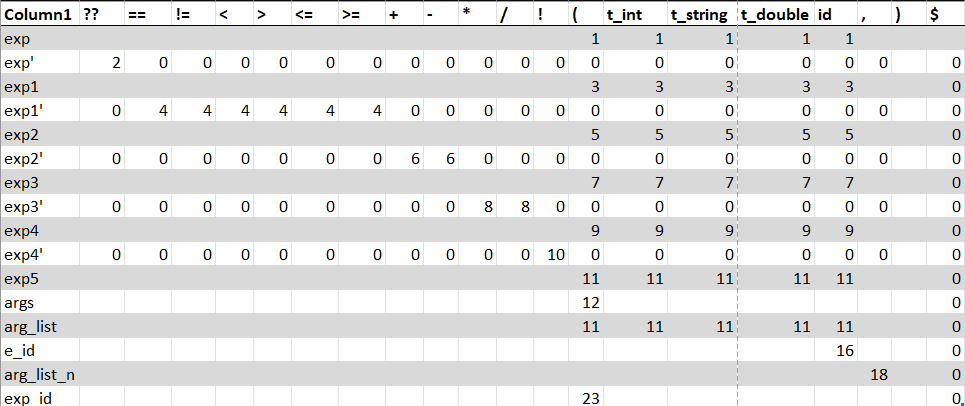
\includegraphics[width=0.9\linewidth]{img/LL-table.png} \\
		\caption{LL -- tabulka použitá při syntaktické analýze}
		\label{table:ll_table}
	\end{table}

\subsection{Sémantická analýza}
\subfile{sections/semantic.tex}

\subsection{Generátor vnitřního kódu}
\subfile{sections/ir.tex}

\subsection{Generátor cílového kódu}
\subfile{sections/code_generator.tex}

 \subsection{odchylky od přednášené látky}
    tabulka symbolů drží pouze symboly\\
    propagace typů je změněná \\
    sémantická analýza používá tabulku funkcí a zásobník tabulek proměnných\\    

\subsection{Popis struktur}
\subsubsection{AST}

\subsubsection{Expression}

\subsubsection{Statement}

\subsubsection{VarTable}
Existuje jeden globální VarTable a následně se na VarTableStack přidávají VarTables jednotlivých rámců.
\subsubsection{VarTableStack}

\subsubsection{FuncTable}

    
\clearpage

\section{Práce v týmu}
\subsection{Způsob práce v týmu}
Na projektu se začalo pracovat na konci září, kdy jsme si rozdělili práce mezi jednotlivé členy týmu, vybrali verzovací systém, testovací nástroj. Přibližně do listopadu na jednotlivých částech se pracovalo převážně samostatně, podle počátečního rozdělení, kdy Radek Jestřabík měl za úkol syntakticou analýzu, Ondřej Hruboš sémantickou analýzu, Dominik Borek generátor vnitřního a cílového kódu a Ondřej Šatinský lexikální analýzu. Na začátku listopadu jsme se začali pravidelně scházet a řešit kód, který byl do této fáze implementován. V tuto chvíli na jednotlivých částech pracovali většinou 2 členové týmu, případně celý tým, pokud byl problém a odstraňovaly se chyby v jednotlivých částech projektu.

\subsection{Rozdělení práce}
\begin{table}[ht]
		\centering
		\begin{tabular}{| c | c |}
			\hline
			Člen týmu & Přidělená práce \\ 
                \hline
			Dominik Borek & \begin{tabular}{c} 
                        sémantická analýza, psaní dokumentace,   fungování LL gramatiky, testování
                     \end{tabular} 
                \\ 
                    
			\textbf{Ondřej Hruboš} & \begin{tabular}{c} 
                        rozbor výrazů, tvorba struktur, makefile, testování
                    \end{tabular} 
                    \\

			Radek Jestřabík & \begin{tabular}{c} 
                        syntaktická analýza, sémantická analýza, testování
                     \end{tabular} 
                     \\
                     
			Ondřej Šatinský & \begin{tabular}{c} 
                        lexikální analýza, generátor kódu, fungování LL gramatiky, testování
                     \end{tabular}  
            \\ \hline
		\end{tabular}
		\caption{Rozdělení práce v týmu mezi jednotlivými členy}
		\label{table:rozdeleni_prace}
	\end{table}


%=============================================================================%
% ZADÁNÍ
%=============================================================================%
%V dokumentaci popisujte návrh (části překladače a předávání informací mezi nimi),
%implementaci (použité datové struktury, tabulku symbolů, generování kódu), vývojový cyk-
%lus, způsob práce v týmu, speciální použité techniky a algoritmy a různé odchylky od před-
%nášené látky či tradičních přístupů. Nezapomínejte také citovat literaturu a uvádět refe-
%rence na čerpané zdroje včetně správné citace převzatých částí (obrázky, magické konstanty,
%vzorce). Nepopisujte záležitosti obecně známé či přednášené na naší fakultě.
%Dokumentace musí povinně obsahovat (povinné tabulky a diagramy se nezapočítá-
%vají do doporučeného rozsahu):
%• 1. strana: jména, příjmení a přihlašovací jména řešitelů (označení vedoucího) + údaje
%o rozdělení bodů, identifikaci vaší varianty zadání ve tvaru “Tým login_vedoucího,
%varianta ��” a výčet identifikátorů implementovaných rozšíření.
%• Rozdělení práce mezi členy týmu (uveďte kdo a jak se podílel na jednotlivých částech
%projektu; povinně zdůvodněte odchylky od rovnoměrného rozdělení bodů).
%• Diagram konečného automatu, který specifikuje lexikální analyzátor.
%• LL-gramatiku, LL-tabulku a precedenční tabulku, podle kterých jste implementovali
%váš syntaktický analyzátor.
%• Stručný popis členění implementačního řešení včetně názvů souborů, kde jsou jed-
%notlivé části včetně povinných implementovaných metod překladače k nalezení

% ZATÍM POUŽITY PRACOVNÍ NÁZVY PRO SEKCE
\end{document}